Trust is widely recognized as a critical part of %interpersonal relationships which affects 
intelligent multi-agent system dynamics---from those involving only simple one-on-one interactions \cite{Lewicki2006-hj}, to more complex ones describing markets and governments \cite{Fukuyama1995-un}. 
Because of interest spanning many disciplines, it is difficult (if not impossible) to write a succinct definition of trust that would completely satisfy all interested parties. 
However, following \cite{McKnight2004-vv}, for the purposes of this work trust is defined here as a psychological state in which an agent willingly and securely becomes vulnerable, or depends on, a trustee (e.g., another person, institution, or an AIA), having taken into consideration the characteristics (e.g., benevolence, integrity, competence) of the trustee. 

This raises two important questions. Firstly, since trust is generally understood to exist between people, is it possible for a human to enter into a trusting relationship with an AIA? 
That humans actually do develop trust in autonomous machines has been confirmed several times~\cite{Muir1996-gt,Mcknight2011-gv,Riley1996-qm,Bainbridge2011-pl,Salem2015-md,Desai2012-rc, Freedy2007-sg, Kaniarasu2013-ho, Wang2016-id}. 
\citet{Lacher2014-yc} also notes that people trust AIAs for transportation systems at different levels (i.e. an engineer trusts differently than an operator or passenger). 
Secondly, in designing assurances that affect trust-based user behaviors, is it possible to know what drives those behaviors and thus have some working model of user trust that can be mapped to AIAs? 
\citet{McKnight1998-ty} (and later \cite{McKnight2001-fa}) performed what is arguably the first multi-disciplinary survey and unification of trust literature, which also condensed it into a single typology consisting of four major related components. 
Adapted to AIAs, these are: \textit{Disposition to Trust:} the extent to which one displays a tendency to be willing to depend on AIAs in general across a broad spectrum of situations and persons; \textit{Institution-Based Trust:} the extent to which one believes that regulations are in place that are conducive to situational success in an endeavor; \textit{Trusting Beliefs:} the extent to which one believes that the AIA has one or more characteristics beneficial to oneself; \textit{Trusting Intentions:} the extent to which one is willing to depend on, or intends to depend on, the AIA even though one cannot control its every action. 
Dispositional Trust is generally considered by psychologists, and deals with long-term psychological traits that develop in a person from childhood (e.g. is someone pre-disposed to trusting technology?).  
Institutional Trust 
is generally studied by sociologists, and represents the level to which a person trusts social/commercial structures. 
Finally, Interpersonal Trust (encompassing both `trusting beliefs', and `trusting intentions') deals directly with one-on-one relationships and tends to fluctuate most quickly. 
Each of these trust components has sub-components defined in Figure~\ref{fig:Assurance_classes}, which were identified by compiling many research studies across several disciplines. 
These components are the principal drivers of user trust-related behaviors, and are the general notional targets of AIA assurances.

\begin{figure}[t]%[htbp]
    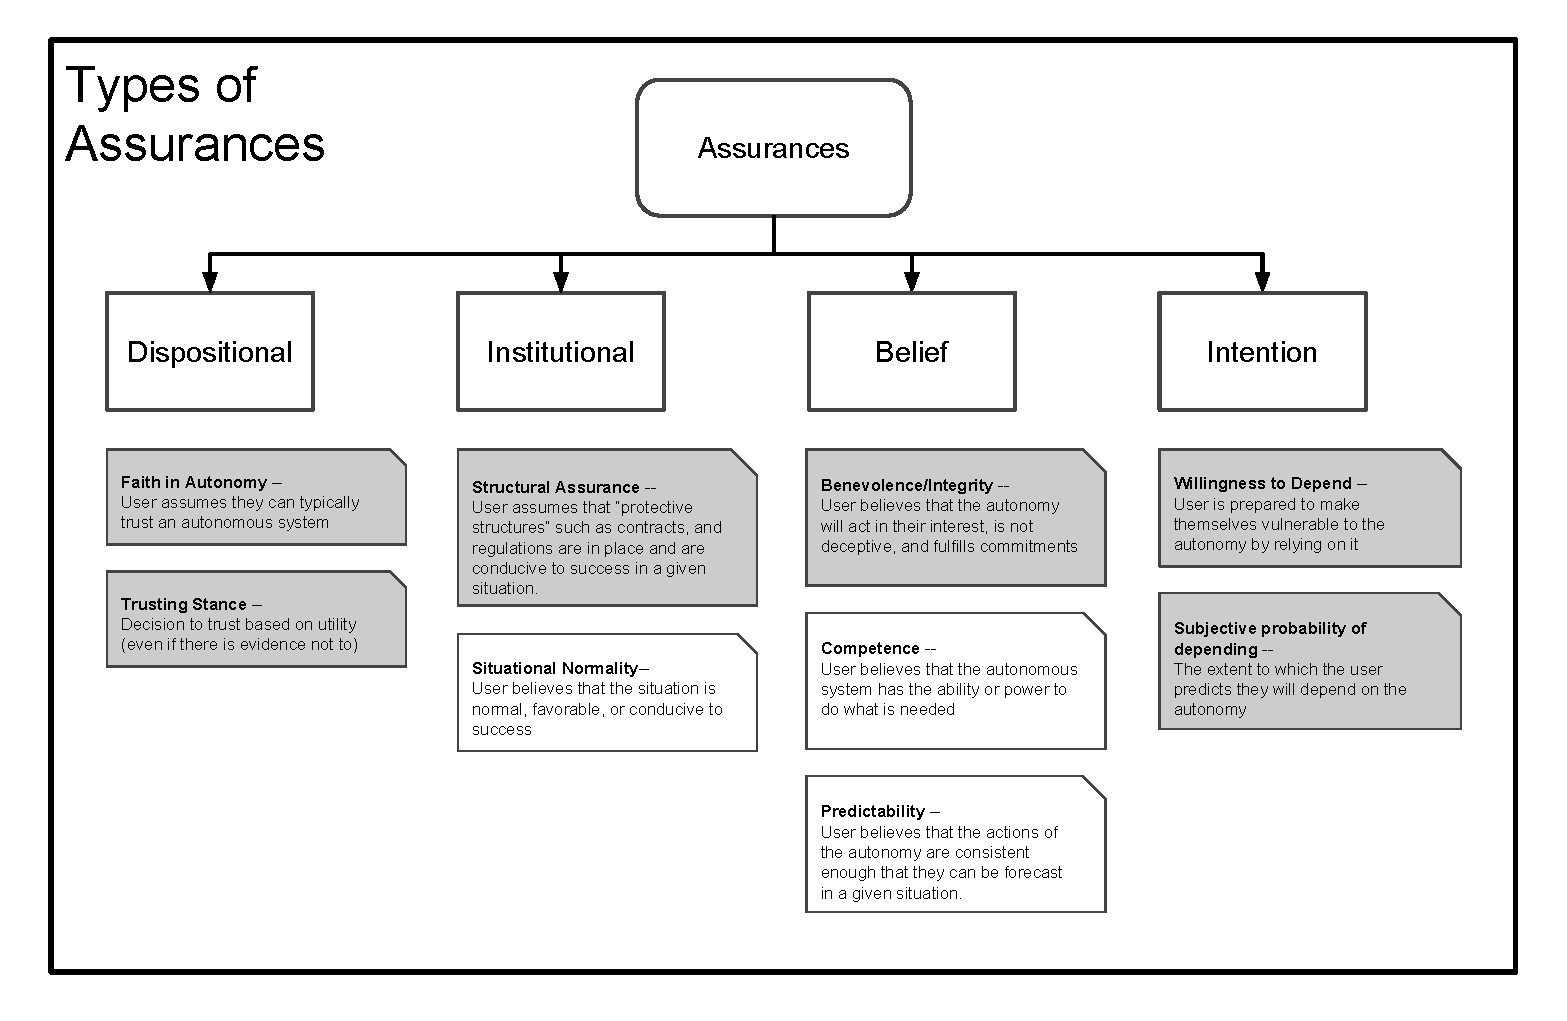
\includegraphics[width=0.95\textwidth]{Figures/Assurances.pdf}%
    \caption{Notional assurance targets based on the component definitions of the main trust categories. While any of these could be considered targets for assurances, the focus here is only on `Situational Normality', `Competence', and `Predictability'.}
    \label{fig:Assurance_classes}
    \vspace{-0.2 in}
\end{figure}
